% Options for packages loaded elsewhere
\PassOptionsToPackage{unicode}{hyperref}
\PassOptionsToPackage{hyphens}{url}
\PassOptionsToPackage{dvipsnames,svgnames,x11names}{xcolor}
%
\documentclass[
  letterpaper,
  DIV=11,
  numbers=noendperiod]{scrartcl}

\usepackage{amsmath,amssymb}
\usepackage{lmodern}
\usepackage{iftex}
\ifPDFTeX
  \usepackage[T1]{fontenc}
  \usepackage[utf8]{inputenc}
  \usepackage{textcomp} % provide euro and other symbols
\else % if luatex or xetex
  \usepackage{unicode-math}
  \defaultfontfeatures{Scale=MatchLowercase}
  \defaultfontfeatures[\rmfamily]{Ligatures=TeX,Scale=1}
\fi
% Use upquote if available, for straight quotes in verbatim environments
\IfFileExists{upquote.sty}{\usepackage{upquote}}{}
\IfFileExists{microtype.sty}{% use microtype if available
  \usepackage[]{microtype}
  \UseMicrotypeSet[protrusion]{basicmath} % disable protrusion for tt fonts
}{}
\makeatletter
\@ifundefined{KOMAClassName}{% if non-KOMA class
  \IfFileExists{parskip.sty}{%
    \usepackage{parskip}
  }{% else
    \setlength{\parindent}{0pt}
    \setlength{\parskip}{6pt plus 2pt minus 1pt}}
}{% if KOMA class
  \KOMAoptions{parskip=half}}
\makeatother
\usepackage{xcolor}
\setlength{\emergencystretch}{3em} % prevent overfull lines
\setcounter{secnumdepth}{5}
% Make \paragraph and \subparagraph free-standing
\ifx\paragraph\undefined\else
  \let\oldparagraph\paragraph
  \renewcommand{\paragraph}[1]{\oldparagraph{#1}\mbox{}}
\fi
\ifx\subparagraph\undefined\else
  \let\oldsubparagraph\subparagraph
  \renewcommand{\subparagraph}[1]{\oldsubparagraph{#1}\mbox{}}
\fi

\usepackage{color}
\usepackage{fancyvrb}
\newcommand{\VerbBar}{|}
\newcommand{\VERB}{\Verb[commandchars=\\\{\}]}
\DefineVerbatimEnvironment{Highlighting}{Verbatim}{commandchars=\\\{\}}
% Add ',fontsize=\small' for more characters per line
\usepackage{framed}
\definecolor{shadecolor}{RGB}{241,243,245}
\newenvironment{Shaded}{\begin{snugshade}}{\end{snugshade}}
\newcommand{\AlertTok}[1]{\textcolor[rgb]{0.68,0.00,0.00}{#1}}
\newcommand{\AnnotationTok}[1]{\textcolor[rgb]{0.37,0.37,0.37}{#1}}
\newcommand{\AttributeTok}[1]{\textcolor[rgb]{0.40,0.45,0.13}{#1}}
\newcommand{\BaseNTok}[1]{\textcolor[rgb]{0.68,0.00,0.00}{#1}}
\newcommand{\BuiltInTok}[1]{\textcolor[rgb]{0.00,0.23,0.31}{#1}}
\newcommand{\CharTok}[1]{\textcolor[rgb]{0.13,0.47,0.30}{#1}}
\newcommand{\CommentTok}[1]{\textcolor[rgb]{0.37,0.37,0.37}{#1}}
\newcommand{\CommentVarTok}[1]{\textcolor[rgb]{0.37,0.37,0.37}{\textit{#1}}}
\newcommand{\ConstantTok}[1]{\textcolor[rgb]{0.56,0.35,0.01}{#1}}
\newcommand{\ControlFlowTok}[1]{\textcolor[rgb]{0.00,0.23,0.31}{#1}}
\newcommand{\DataTypeTok}[1]{\textcolor[rgb]{0.68,0.00,0.00}{#1}}
\newcommand{\DecValTok}[1]{\textcolor[rgb]{0.68,0.00,0.00}{#1}}
\newcommand{\DocumentationTok}[1]{\textcolor[rgb]{0.37,0.37,0.37}{\textit{#1}}}
\newcommand{\ErrorTok}[1]{\textcolor[rgb]{0.68,0.00,0.00}{#1}}
\newcommand{\ExtensionTok}[1]{\textcolor[rgb]{0.00,0.23,0.31}{#1}}
\newcommand{\FloatTok}[1]{\textcolor[rgb]{0.68,0.00,0.00}{#1}}
\newcommand{\FunctionTok}[1]{\textcolor[rgb]{0.28,0.35,0.67}{#1}}
\newcommand{\ImportTok}[1]{\textcolor[rgb]{0.00,0.46,0.62}{#1}}
\newcommand{\InformationTok}[1]{\textcolor[rgb]{0.37,0.37,0.37}{#1}}
\newcommand{\KeywordTok}[1]{\textcolor[rgb]{0.00,0.23,0.31}{#1}}
\newcommand{\NormalTok}[1]{\textcolor[rgb]{0.00,0.23,0.31}{#1}}
\newcommand{\OperatorTok}[1]{\textcolor[rgb]{0.37,0.37,0.37}{#1}}
\newcommand{\OtherTok}[1]{\textcolor[rgb]{0.00,0.23,0.31}{#1}}
\newcommand{\PreprocessorTok}[1]{\textcolor[rgb]{0.68,0.00,0.00}{#1}}
\newcommand{\RegionMarkerTok}[1]{\textcolor[rgb]{0.00,0.23,0.31}{#1}}
\newcommand{\SpecialCharTok}[1]{\textcolor[rgb]{0.37,0.37,0.37}{#1}}
\newcommand{\SpecialStringTok}[1]{\textcolor[rgb]{0.13,0.47,0.30}{#1}}
\newcommand{\StringTok}[1]{\textcolor[rgb]{0.13,0.47,0.30}{#1}}
\newcommand{\VariableTok}[1]{\textcolor[rgb]{0.07,0.07,0.07}{#1}}
\newcommand{\VerbatimStringTok}[1]{\textcolor[rgb]{0.13,0.47,0.30}{#1}}
\newcommand{\WarningTok}[1]{\textcolor[rgb]{0.37,0.37,0.37}{\textit{#1}}}

\providecommand{\tightlist}{%
  \setlength{\itemsep}{0pt}\setlength{\parskip}{0pt}}\usepackage{longtable,booktabs,array}
\usepackage{calc} % for calculating minipage widths
% Correct order of tables after \paragraph or \subparagraph
\usepackage{etoolbox}
\makeatletter
\patchcmd\longtable{\par}{\if@noskipsec\mbox{}\fi\par}{}{}
\makeatother
% Allow footnotes in longtable head/foot
\IfFileExists{footnotehyper.sty}{\usepackage{footnotehyper}}{\usepackage{footnote}}
\makesavenoteenv{longtable}
\usepackage{graphicx}
\makeatletter
\def\maxwidth{\ifdim\Gin@nat@width>\linewidth\linewidth\else\Gin@nat@width\fi}
\def\maxheight{\ifdim\Gin@nat@height>\textheight\textheight\else\Gin@nat@height\fi}
\makeatother
% Scale images if necessary, so that they will not overflow the page
% margins by default, and it is still possible to overwrite the defaults
% using explicit options in \includegraphics[width, height, ...]{}
\setkeys{Gin}{width=\maxwidth,height=\maxheight,keepaspectratio}
% Set default figure placement to htbp
\makeatletter
\def\fps@figure{htbp}
\makeatother

\KOMAoption{captions}{tableheading}
\makeatletter
\makeatother
\makeatletter
\makeatother
\makeatletter
\@ifpackageloaded{caption}{}{\usepackage{caption}}
\AtBeginDocument{%
\ifdefined\contentsname
  \renewcommand*\contentsname{Table of contents}
\else
  \newcommand\contentsname{Table of contents}
\fi
\ifdefined\listfigurename
  \renewcommand*\listfigurename{List of Figures}
\else
  \newcommand\listfigurename{List of Figures}
\fi
\ifdefined\listtablename
  \renewcommand*\listtablename{List of Tables}
\else
  \newcommand\listtablename{List of Tables}
\fi
\ifdefined\figurename
  \renewcommand*\figurename{Figure}
\else
  \newcommand\figurename{Figure}
\fi
\ifdefined\tablename
  \renewcommand*\tablename{Table}
\else
  \newcommand\tablename{Table}
\fi
}
\@ifpackageloaded{float}{}{\usepackage{float}}
\floatstyle{ruled}
\@ifundefined{c@chapter}{\newfloat{codelisting}{h}{lop}}{\newfloat{codelisting}{h}{lop}[chapter]}
\floatname{codelisting}{Listing}
\newcommand*\listoflistings{\listof{codelisting}{List of Listings}}
\makeatother
\makeatletter
\@ifpackageloaded{caption}{}{\usepackage{caption}}
\@ifpackageloaded{subcaption}{}{\usepackage{subcaption}}
\makeatother
\makeatletter
\@ifpackageloaded{tcolorbox}{}{\usepackage[many]{tcolorbox}}
\makeatother
\makeatletter
\@ifundefined{shadecolor}{\definecolor{shadecolor}{rgb}{.97, .97, .97}}
\makeatother
\makeatletter
\makeatother
\ifLuaTeX
  \usepackage{selnolig}  % disable illegal ligatures
\fi
\IfFileExists{bookmark.sty}{\usepackage{bookmark}}{\usepackage{hyperref}}
\IfFileExists{xurl.sty}{\usepackage{xurl}}{} % add URL line breaks if available
\urlstyle{same} % disable monospaced font for URLs
\hypersetup{
  pdftitle={UW STATR 501A - Homework \#4},
  pdfauthor={Melissa Gaughan},
  colorlinks=true,
  linkcolor={blue},
  filecolor={Maroon},
  citecolor={Blue},
  urlcolor={Blue},
  pdfcreator={LaTeX via pandoc}}

\title{UW STATR 501A - Homework \#4}
\author{Melissa Gaughan}
\date{2022-10-27}

\begin{document}
\maketitle
\ifdefined\Shaded\renewenvironment{Shaded}{\begin{tcolorbox}[breakable, interior hidden, enhanced, boxrule=0pt, frame hidden, borderline west={3pt}{0pt}{shadecolor}, sharp corners]}{\end{tcolorbox}}\fi

\renewcommand*\contentsname{Table of contents}
{
\hypersetup{linkcolor=}
\setcounter{tocdepth}{3}
\tableofcontents
}
\hypertarget{instructions}{%
\section{Instructions}\label{instructions}}

Please submit a single zipped folder with all associated files {[}text
report (.pdf, .docx, .txt), R code (.R, .Rmd), data files (.csv, .xlsx,
.txt){]}. Upload the completed homework assignment into the Canvas
drop-box.

Probability problems may be unintuitive - hence the emphasis on
simulation. Please discuss the problems amongst yourselves on the forum,
but make sure to submit your own work (code and text).

\hypertarget{problem-1---reading}{%
\subsection{Problem \#1 - Reading}\label{problem-1---reading}}

\hypertarget{part-a}{%
\subsubsection{Part a}\label{part-a}}

Read the file lab4\_corrected.html (under modules of the course site)

\hypertarget{part-b}{%
\subsubsection{Part b}\label{part-b}}

Read Ch. 1 Probability Models and Ch. 2 Random Variables and
Distributions in Probability and Statistics.

\hypertarget{part-c}{%
\subsubsection{Part c}\label{part-c}}

Read Ch. 8 Probability Distributions in An Introduction to R.

\hypertarget{problem-2---random-variables-i}{%
\subsection{Problem \#2 - Random Variables
I}\label{problem-2---random-variables-i}}

\hypertarget{part-a-1}{%
\subsubsection{Part a}\label{part-a-1}}

Simulate 1000 numbers from the
\href{https://en.wikipedia.org/wiki/Continuous_uniform_distribution}{standard
uniform distribution} \(X \sim Unif(0,1)\), and report the
\href{https://en.wikipedia.org/wiki/Standard_deviation\#Sample_standard_deviation}{sample
standard deviation} (\(s_{x}\)) of these numbers.

\begin{Shaded}
\begin{Highlighting}[]
\CommentTok{\#\textless{}Write code here\textgreater{}}

\NormalTok{sample\_1000 }\OtherTok{\textless{}{-}} \FunctionTok{runif}\NormalTok{(}\DecValTok{1000}\NormalTok{)}

\NormalTok{standard\_deviation }\OtherTok{\textless{}{-}} \FunctionTok{sqrt}\NormalTok{(}\FunctionTok{var}\NormalTok{(sample\_1000))}
\end{Highlighting}
\end{Shaded}

\hypertarget{part-b-1}{%
\subsubsection{Part b}\label{part-b-1}}

Write a function that returns \(s_{x}\) of \(n\) draws from a
\(Unif(0,b)\) distribution, where \(b\) is the upper limit

\begin{Shaded}
\begin{Highlighting}[]
\CommentTok{\#\textless{}Write code here\textgreater{}}

\NormalTok{standard\_deviation\_function }\OtherTok{\textless{}{-}} \ControlFlowTok{function}\NormalTok{(}\AttributeTok{n =} \DecValTok{1000}\NormalTok{, }\AttributeTok{upper\_limit =} \DecValTok{1}\NormalTok{)\{}
\NormalTok{  sample }\OtherTok{\textless{}{-}} \FunctionTok{runif}\NormalTok{(}\AttributeTok{n =}\NormalTok{ n, }
                    \AttributeTok{min =} \DecValTok{0}\NormalTok{, }
                    \AttributeTok{max =}\NormalTok{ upper\_limit)}

\NormalTok{standard\_deviation }\OtherTok{\textless{}{-}} \FunctionTok{sqrt}\NormalTok{(}\FunctionTok{var}\NormalTok{(sample))}

\FunctionTok{return}\NormalTok{(standard\_deviation)}
  
\NormalTok{\}}


\FunctionTok{standard\_deviation\_function}\NormalTok{(}\AttributeTok{n =} \DecValTok{50}\NormalTok{, }\AttributeTok{upper\_limit =} \DecValTok{500}\NormalTok{)}
\end{Highlighting}
\end{Shaded}

\begin{verbatim}
[1] 143.4184
\end{verbatim}

\hypertarget{part-c-1}{%
\subsubsection{Part c}\label{part-c-1}}

Obtain the values \(s_{x}\) against values of \(b\) ranging from 1 to 10
(using any large value of \(n\) of your choosing). Is there a consistent
pattern? Can you propose a model that predicts \(s_{x}\) with upper
limit \(b\)?

\begin{Shaded}
\begin{Highlighting}[]
\NormalTok{results }\OtherTok{\textless{}{-}} \FunctionTok{rep}\NormalTok{(}\FunctionTok{as.numeric}\NormalTok{(}\ConstantTok{NA}\NormalTok{), }\DecValTok{10}\NormalTok{)}
\CommentTok{\#\textless{}Write code here\textgreater{}}

\ControlFlowTok{for}\NormalTok{ (i }\ControlFlowTok{in} \FunctionTok{seq}\NormalTok{(}\DecValTok{1}\SpecialCharTok{:}\DecValTok{10}\NormalTok{))\{}
\NormalTok{  test }\OtherTok{\textless{}{-}} \FunctionTok{standard\_deviation\_function}\NormalTok{(}\AttributeTok{n =} \DecValTok{10000}\NormalTok{, }\AttributeTok{upper\_limit =}\NormalTok{ i)}
\NormalTok{  results[i] }\OtherTok{\textless{}{-}}\NormalTok{ test}
\NormalTok{\}}

\NormalTok{results}
\end{Highlighting}
\end{Shaded}

\begin{verbatim}
 [1] 0.2915706 0.5812578 0.8758322 1.1604039 1.4361345 1.7335944 2.0135039
 [8] 2.3088719 2.5914054 2.9074487
\end{verbatim}

\begin{Shaded}
\begin{Highlighting}[]
\NormalTok{results[}\DecValTok{1}\NormalTok{] }\SpecialCharTok{{-}}\NormalTok{ results[}\DecValTok{2}\NormalTok{]}
\end{Highlighting}
\end{Shaded}

\begin{verbatim}
[1] -0.2896871
\end{verbatim}

\begin{Shaded}
\begin{Highlighting}[]
\NormalTok{results[}\DecValTok{2}\NormalTok{] }\SpecialCharTok{{-}}\NormalTok{ results[}\DecValTok{3}\NormalTok{]}
\end{Highlighting}
\end{Shaded}

\begin{verbatim}
[1] -0.2945744
\end{verbatim}

\begin{Shaded}
\begin{Highlighting}[]
\NormalTok{results[}\DecValTok{3}\NormalTok{] }\SpecialCharTok{{-}}\NormalTok{ results[}\DecValTok{4}\NormalTok{]}
\end{Highlighting}
\end{Shaded}

\begin{verbatim}
[1] -0.2845717
\end{verbatim}

\begin{Shaded}
\begin{Highlighting}[]
\NormalTok{results[}\DecValTok{4}\NormalTok{] }\SpecialCharTok{{-}}\NormalTok{ results[}\DecValTok{5}\NormalTok{]}
\end{Highlighting}
\end{Shaded}

\begin{verbatim}
[1] -0.2757306
\end{verbatim}

\begin{Shaded}
\begin{Highlighting}[]
\FloatTok{0.288} \SpecialCharTok{+} \DecValTok{11}\SpecialCharTok{*}\NormalTok{.}\DecValTok{288}
\end{Highlighting}
\end{Shaded}

\begin{verbatim}
[1] 3.456
\end{verbatim}

\begin{Shaded}
\begin{Highlighting}[]
\DecValTok{10}\SpecialCharTok{*}\NormalTok{.}\DecValTok{288}
\end{Highlighting}
\end{Shaded}

\begin{verbatim}
[1] 2.88
\end{verbatim}

\begin{Shaded}
\begin{Highlighting}[]
\DecValTok{11}\SpecialCharTok{*}\NormalTok{.}\DecValTok{288}
\end{Highlighting}
\end{Shaded}

\begin{verbatim}
[1] 3.168
\end{verbatim}

The results sample standard deviation seems to increase by approximately
0.288 as the upper limit increases by 1. I would propose that the
standard deviation could be predicted by multiplying the upper limit by
0.288.

\hypertarget{problem-3---random-variables-ii}{%
\subsection{Problem \#3 - Random Variables
II}\label{problem-3---random-variables-ii}}

\hypertarget{part-a-2}{%
\subsubsection{Part a}\label{part-a-2}}

Generate two vectors \(X_{1}\) and \(X_{2}\), each of which represents
10,000 draws from the \(Unif(0,1)\) distribution. Obtain the pairwise
sum of these vectors (\(Y_{2} = X_{1} + X_{2}\)) and plot the density
histogram of \(Y\).

\begin{Shaded}
\begin{Highlighting}[]
\CommentTok{\#\textless{}Write code here\textgreater{}}

\NormalTok{sample\_1 }\OtherTok{\textless{}{-}} \FunctionTok{runif}\NormalTok{(}\AttributeTok{n =} \DecValTok{10000}\NormalTok{, }
                    \AttributeTok{min =} \DecValTok{0}\NormalTok{, }
                    \AttributeTok{max =} \DecValTok{1}\NormalTok{)}
 
\NormalTok{sample\_2 }\OtherTok{\textless{}{-}} \FunctionTok{runif}\NormalTok{(}\AttributeTok{n =} \DecValTok{10000}\NormalTok{, }
                    \AttributeTok{min =} \DecValTok{0}\NormalTok{, }
                    \AttributeTok{max =} \DecValTok{1}\NormalTok{)}
\NormalTok{combined\_sample }\OtherTok{\textless{}{-}}\NormalTok{ sample\_1}\SpecialCharTok{+}\NormalTok{sample\_2}

\NormalTok{data }\OtherTok{\textless{}{-}} \FunctionTok{as\_tibble}\NormalTok{(combined\_sample)}

\NormalTok{density\_plot }\OtherTok{\textless{}{-}}  
\NormalTok{  ggplot2}\SpecialCharTok{::}\FunctionTok{ggplot}\NormalTok{(data)}\SpecialCharTok{+}
\NormalTok{  ggplot2}\SpecialCharTok{::}\FunctionTok{geom\_density}\NormalTok{(}\FunctionTok{aes}\NormalTok{(}\AttributeTok{x=}\NormalTok{ value))}

\NormalTok{density\_plot}
\end{Highlighting}
\end{Shaded}

\begin{figure}[H]

{\centering 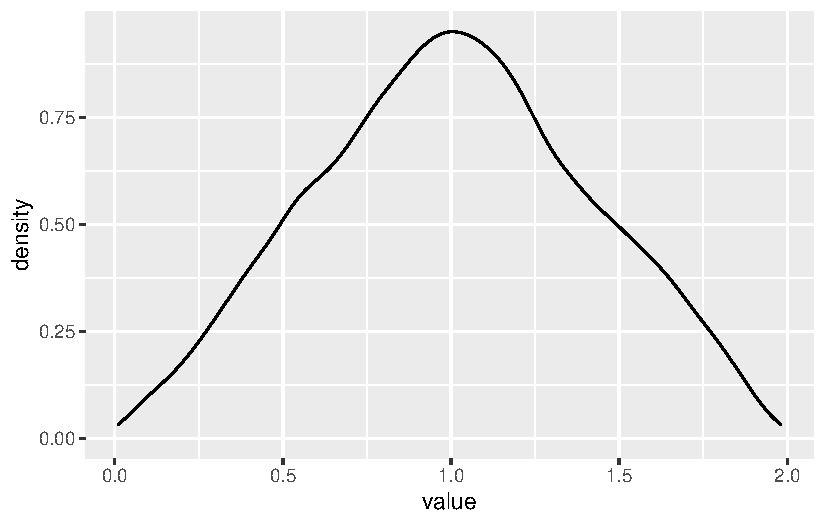
\includegraphics{HW04_Gaughan_Melissa_files/figure-pdf/3a-1.pdf}

}

\end{figure}

\hypertarget{part-b-2}{%
\subsubsection{Part b}\label{part-b-2}}

Guess what the probability distribution function (p.d.f.) of \(Y_{2}\)
might be (i.e.~describe it mathematically with a pairwise function), and
illustrate it with a line over the histogram.

\begin{Shaded}
\begin{Highlighting}[]
\FunctionTok{hist}\NormalTok{(combined\_sample, }\AttributeTok{probability =} \ConstantTok{TRUE}\NormalTok{, }\AttributeTok{xaxs =} \StringTok{"i"}\NormalTok{, }\AttributeTok{yaxs =} \StringTok{"i"}\NormalTok{, }\AttributeTok{ylim =} \FunctionTok{c}\NormalTok{(}\DecValTok{0}\NormalTok{, }\DecValTok{1}\NormalTok{))}
\FunctionTok{lines}\NormalTok{(}\FunctionTok{c}\NormalTok{(}\SpecialCharTok{{-}}\DecValTok{10}\NormalTok{, }\DecValTok{0}\NormalTok{, }\DecValTok{1}\NormalTok{, }\DecValTok{2}\NormalTok{, }\DecValTok{10}\NormalTok{), }\FunctionTok{c}\NormalTok{(}\DecValTok{0}\NormalTok{, }\DecValTok{0}\NormalTok{, }\DecValTok{1}\NormalTok{, }\DecValTok{0}\NormalTok{, }\DecValTok{0}\NormalTok{))}
\end{Highlighting}
\end{Shaded}

\begin{figure}[H]

{\centering 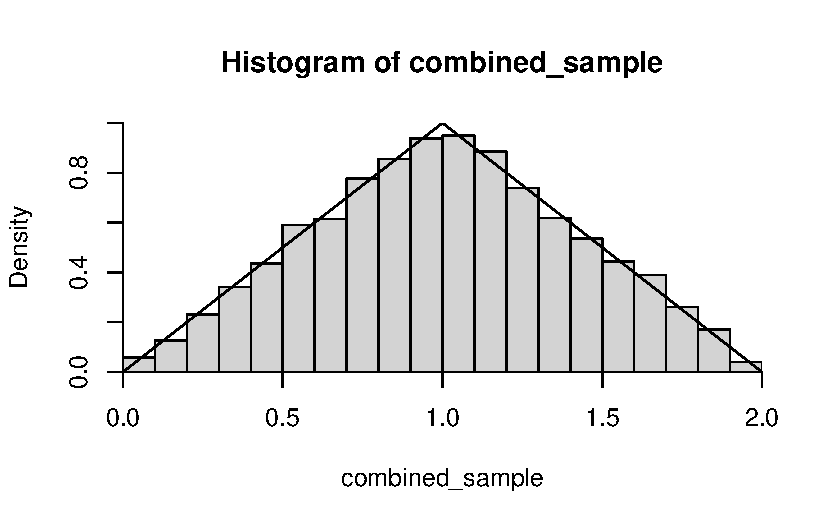
\includegraphics{HW04_Gaughan_Melissa_files/figure-pdf/3b-1.pdf}

}

\end{figure}

\hypertarget{part-c-2}{%
\subsubsection{Part c}\label{part-c-2}}

Similarly, obtain \(Y_{5} = X_{1} + X_{2} + ... + X_{5}\) and
\(Y_{10}\). Plot on a single 4x2 figure the respective histograms and
qqnorm plots of \(X_{1}, Y_{2}, Y_{5}, Y_{10}\). What do you observe?

\begin{Shaded}
\begin{Highlighting}[]
\CommentTok{\#\textless{}Write code here\textgreater{}}


\NormalTok{combined\_sample\_5 }\OtherTok{\textless{}{-}} \FunctionTok{runif}\NormalTok{(}\DecValTok{10000}\NormalTok{, }\DecValTok{0}\NormalTok{, }\DecValTok{1}\NormalTok{)}
\ControlFlowTok{for}\NormalTok{ (i }\ControlFlowTok{in} \DecValTok{2}\SpecialCharTok{:}\DecValTok{5}\NormalTok{) \{}
\NormalTok{  combined\_sample\_5 }\OtherTok{\textless{}{-}}\NormalTok{ combined\_sample\_5 }\SpecialCharTok{+} \FunctionTok{runif}\NormalTok{(}\DecValTok{10000}\NormalTok{, }\DecValTok{0}\NormalTok{, }\DecValTok{1}\NormalTok{)}
\NormalTok{\}}

\NormalTok{combined\_sample\_10 }\OtherTok{\textless{}{-}} \FunctionTok{runif}\NormalTok{(}\DecValTok{10000}\NormalTok{, }\DecValTok{0}\NormalTok{, }\DecValTok{1}\NormalTok{)}
\ControlFlowTok{for}\NormalTok{ (i }\ControlFlowTok{in} \DecValTok{2}\SpecialCharTok{:}\DecValTok{5}\NormalTok{) \{}
\NormalTok{  combined\_sample\_10 }\OtherTok{\textless{}{-}}\NormalTok{ combined\_sample\_10 }\SpecialCharTok{+} \FunctionTok{runif}\NormalTok{(}\DecValTok{10000}\NormalTok{, }\DecValTok{0}\NormalTok{, }\DecValTok{1}\NormalTok{)}
\NormalTok{\}}

\NormalTok{tibble\_1 }\OtherTok{\textless{}{-}} \FunctionTok{as\_tibble}\NormalTok{(sample\_1)}

\NormalTok{tibble\_2 }\OtherTok{\textless{}{-}} \FunctionTok{as\_tibble}\NormalTok{(combined\_sample)}

\NormalTok{tibble\_5 }\OtherTok{\textless{}{-}} \FunctionTok{as\_tibble}\NormalTok{(combined\_sample\_5)}

\NormalTok{tibble\_10 }\OtherTok{\textless{}{-}} \FunctionTok{as\_tibble}\NormalTok{(combined\_sample\_10)}
\NormalTok{tables }\OtherTok{\textless{}{-}} \FunctionTok{list}\NormalTok{(tibble\_1, tibble\_2, tibble\_5, tibble\_10)}

\ControlFlowTok{for}\NormalTok{(i }\ControlFlowTok{in} \FunctionTok{seq\_along}\NormalTok{(tables))\{}
 \CommentTok{\# i = 1}
\NormalTok{  density\_plot }\OtherTok{\textless{}{-}}\NormalTok{  ggplot2}\SpecialCharTok{::}\FunctionTok{ggplot}\NormalTok{(tables[[i]])}\SpecialCharTok{+}
\NormalTok{  ggplot2}\SpecialCharTok{::}\FunctionTok{geom\_density}\NormalTok{(}\FunctionTok{aes}\NormalTok{(}\AttributeTok{x=}\NormalTok{ value))}\SpecialCharTok{+}
  \FunctionTok{labs}\NormalTok{(}\AttributeTok{title =}\StringTok{"Density Plot"}\NormalTok{, }
   
       \AttributeTok{ylab =} \StringTok{"Density"}\NormalTok{)}
  
\NormalTok{  qqplot }\OtherTok{\textless{}{-}}\NormalTok{   ggplot2}\SpecialCharTok{::}\FunctionTok{ggplot}\NormalTok{(tables[[i]])}\SpecialCharTok{+}
\NormalTok{  ggplot2}\SpecialCharTok{::}\FunctionTok{geom\_qq}\NormalTok{(}\FunctionTok{aes}\NormalTok{(}\AttributeTok{sample=}\NormalTok{ value)) }\SpecialCharTok{+}
    \FunctionTok{labs}\NormalTok{(}\AttributeTok{title =} \StringTok{"QQ Plot "}\NormalTok{)}
  
  \FunctionTok{print}\NormalTok{( density\_plot }\SpecialCharTok{/}\NormalTok{ qqplot)}


\NormalTok{\}}
\end{Highlighting}
\end{Shaded}

\begin{figure}[H]

{\centering 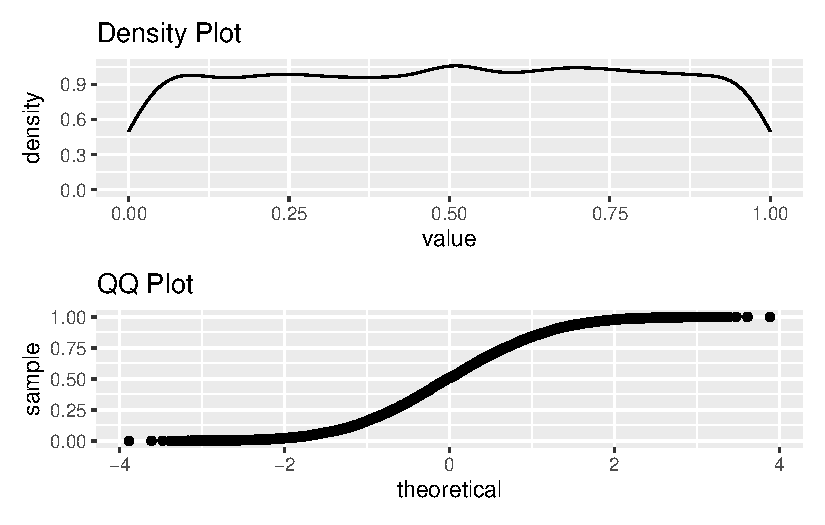
\includegraphics{HW04_Gaughan_Melissa_files/figure-pdf/3c-1.pdf}

}

\end{figure}

\begin{figure}[H]

{\centering 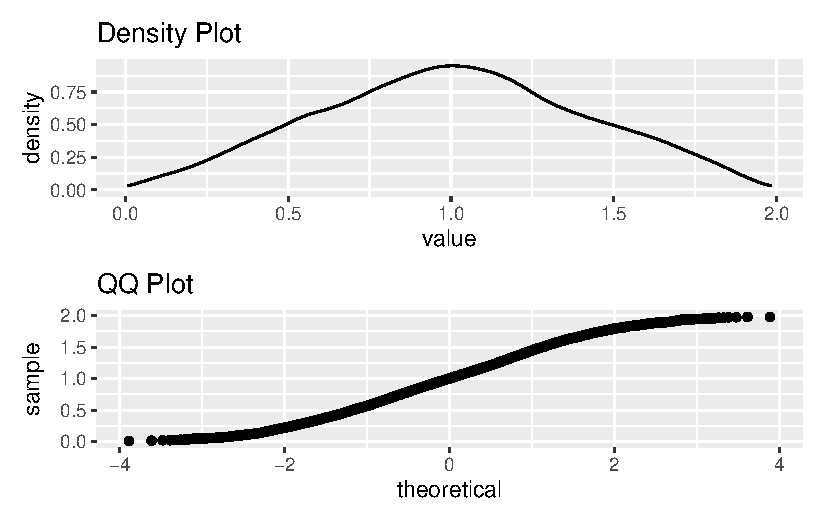
\includegraphics{HW04_Gaughan_Melissa_files/figure-pdf/3c-2.pdf}

}

\end{figure}

\begin{figure}[H]

{\centering 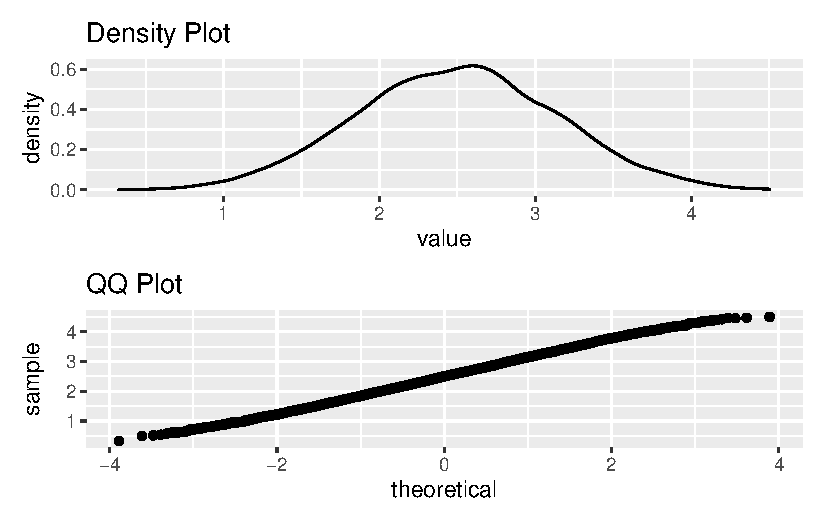
\includegraphics{HW04_Gaughan_Melissa_files/figure-pdf/3c-3.pdf}

}

\end{figure}

\begin{figure}[H]

{\centering 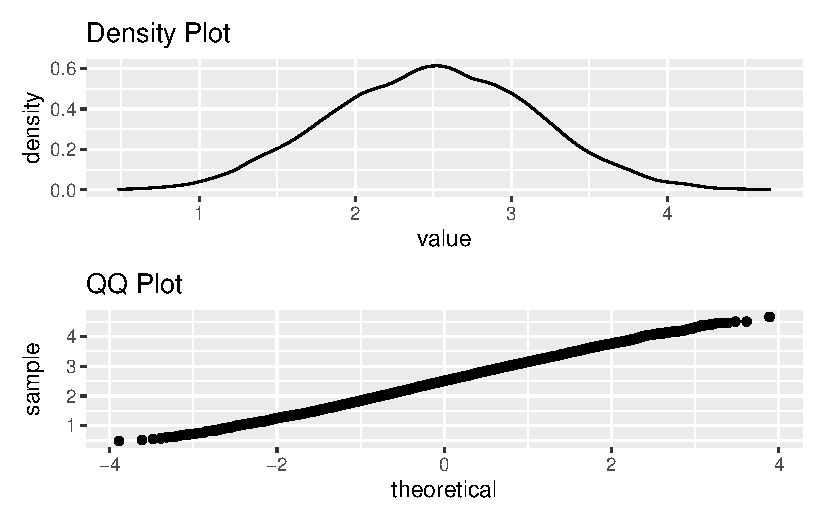
\includegraphics{HW04_Gaughan_Melissa_files/figure-pdf/3c-4.pdf}

}

\end{figure}

As more observations are taken from the normal distribution, the data
becomes more normal (the QQ plot approaches a diagonal line with a
positive slope). This is an example of the Central Limit Theorem.

\hypertarget{problem-4---de-muxe9ruxe9s-wager-i}{%
\subsection{Problem \#4 - De Méré's Wager
I}\label{problem-4---de-muxe9ruxe9s-wager-i}}

\href{https://en.wikipedia.org/wiki/Antoine_Gombaud}{Antoine Gombaud},
a.k.a. the Chevalier de Méré (1607-1684) was a ``gentleman gambler''
(and amateur mathematician) in France. One game de Méré enjoyed playing
(though it sounds awfully boring to me) would be to bet with even odds
(i.e.~lose a franc if you lose, win a franc if you win) on getting at
least one six on four rolls of a fair die. He reasoned that the chance
of getting a six in one roll of a die is \(1/6\), so the chance of
getting one six in four would be \(4/6=2/3\).

\hypertarget{part-a-3}{%
\subsubsection{Part a}\label{part-a-3}}

Write a function \texttt{DeMereA(n)} that simulates this game,
i.e.~takes a certain number \((n)\) of rolls of a die and returns a
\texttt{TRUE} if there is at least one six and a \texttt{FALSE} if there
isn't.

\begin{Shaded}
\begin{Highlighting}[]
\CommentTok{\#\textless{}Write code here\textgreater{}}

\NormalTok{DeMere\_A }\OtherTok{\textless{}{-}} \ControlFlowTok{function}\NormalTok{(}\AttributeTok{number\_rolls =} \DecValTok{10}\NormalTok{)\{}
\NormalTok{  sample }\OtherTok{\textless{}{-}} \FunctionTok{as.vector}\NormalTok{(}\FunctionTok{c}\NormalTok{(1L}\SpecialCharTok{:}\NormalTok{6L))}
  
\NormalTok{    result }\OtherTok{\textless{}{-}} \FunctionTok{sample}\NormalTok{(}\AttributeTok{x =}\NormalTok{ sample, }\AttributeTok{size =}\NormalTok{ number\_rolls, }
                         \AttributeTok{replace =}\NormalTok{ T)}
    
    \ControlFlowTok{if}\NormalTok{( }\DecValTok{6} \SpecialCharTok{\%in\%}\NormalTok{ result)\{}
      \FunctionTok{return}\NormalTok{(}\ConstantTok{TRUE}\NormalTok{)}
\NormalTok{    \} }\ControlFlowTok{else}\NormalTok{ \{}
      \FunctionTok{return}\NormalTok{(}\ConstantTok{FALSE}\NormalTok{)}
\NormalTok{    \}}
\NormalTok{  \}}
\end{Highlighting}
\end{Shaded}

\hypertarget{part-b-3}{%
\subsubsection{Part b}\label{part-b-3}}

Simulate 1000 of these games and compute the number of times he wins.

\begin{Shaded}
\begin{Highlighting}[]
\CommentTok{\#\textless{}Write code here\textgreater{}}


\NormalTok{DeMere\_B }\OtherTok{\textless{}{-}} \ControlFlowTok{function}\NormalTok{(}\AttributeTok{number\_rolls =} \DecValTok{10}\NormalTok{)\{}
\NormalTok{  sample }\OtherTok{\textless{}{-}} \FunctionTok{as.vector}\NormalTok{(}\FunctionTok{c}\NormalTok{(1L}\SpecialCharTok{:}\NormalTok{6L))}
  
\NormalTok{    result }\OtherTok{\textless{}{-}} \FunctionTok{sample}\NormalTok{(}\AttributeTok{x =}\NormalTok{ sample, }\AttributeTok{size =}\NormalTok{ number\_rolls, }
                         \AttributeTok{replace =}\NormalTok{ T)}
    
\NormalTok{    wins }\OtherTok{\textless{}{-}}\NormalTok{ result[result}\SpecialCharTok{==}\DecValTok{6}\NormalTok{]}
    
    \FunctionTok{return}\NormalTok{(}\FunctionTok{length}\NormalTok{(wins))}
    
\NormalTok{\}}

\FunctionTok{DeMere\_B}\NormalTok{(}\AttributeTok{number\_rolls =} \DecValTok{1000}\NormalTok{)}
\end{Highlighting}
\end{Shaded}

\begin{verbatim}
[1] 161
\end{verbatim}

\hypertarget{part-c-3}{%
\subsubsection{Part c}\label{part-c-3}}

De Méré's reasoning was faulty, but he still won a lot of money playing
this (frankly, kind of stupid) game. What is the actual probability of
getting at least one six in four rolls? (Use math or simulate in R)

\begin{Shaded}
\begin{Highlighting}[]
\CommentTok{\#\textless{}Write code here\textgreater{}}

\DecValTok{1}\SpecialCharTok{{-}}\NormalTok{(}\DecValTok{5}\SpecialCharTok{/}\DecValTok{6}\NormalTok{)}\SpecialCharTok{\^{}}\DecValTok{4}
\end{Highlighting}
\end{Shaded}

\begin{verbatim}
[1] 0.5177469
\end{verbatim}

\hypertarget{problem-5---de-muxe9ruxe9s-wager-ii}{%
\subsection{Problem \#5 - De Méré's Wager
II}\label{problem-5---de-muxe9ruxe9s-wager-ii}}

Despite the faulty reasoning, de Méré actually won a lot of money
playing this game but became bored of it. So, to make things mildly more
interesting, he devised a second game. In this one, he would wager -
again with even odds - on getting at least one double six on 24 rolls of
a pair of dice. He reasoned correctly that the chance of getting a
double six in rolling a pair of dice is \(1/36\). So he assumed that in
24 rolls of a pair of dice, the chance of getting one double six would
be \(24/36=2/3\).

\hypertarget{part-a-4}{%
\subsubsection{Part a}\label{part-a-4}}

Write an analogous function \texttt{DeMereB(n)} that simulates the 24
roll game with double dice.

\begin{Shaded}
\begin{Highlighting}[]
\CommentTok{\#\textless{}Write code here\textgreater{}}

\NormalTok{DeMere\_24 }\OtherTok{\textless{}{-}} \ControlFlowTok{function}\NormalTok{(}\AttributeTok{number\_rolls =} \DecValTok{24}\NormalTok{)\{}
\NormalTok{  sample }\OtherTok{\textless{}{-}} \FunctionTok{as.vector}\NormalTok{(}\FunctionTok{c}\NormalTok{(1L}\SpecialCharTok{:}\NormalTok{6L))}
  
\NormalTok{    result\_1 }\OtherTok{\textless{}{-}} \FunctionTok{as\_tibble\_col}\NormalTok{(}\FunctionTok{sample}\NormalTok{(}\AttributeTok{x =}\NormalTok{ sample, }
                                     \AttributeTok{size =}\NormalTok{  number\_rolls, }
                                     \AttributeTok{replace =}\NormalTok{ T), }
                              \AttributeTok{column\_name =} \StringTok{"die\_1"}\NormalTok{)}
    
\NormalTok{    result\_2 }\OtherTok{\textless{}{-}} \FunctionTok{as\_tibble\_col}\NormalTok{(}\FunctionTok{sample}\NormalTok{(}\AttributeTok{x =}\NormalTok{ sample,}
                                     \AttributeTok{size =}\NormalTok{ number\_rolls, }
                                     \AttributeTok{replace =}\NormalTok{ T), }
                              \AttributeTok{column\_name =} \StringTok{"die\_2"}\NormalTok{)}
    
    
    
\NormalTok{    wins\_1 }\OtherTok{\textless{}{-}} \FunctionTok{bind\_cols}\NormalTok{(result\_1, result\_2) }\SpecialCharTok{\%\textgreater{}\%} 
      \FunctionTok{filter}\NormalTok{(die\_1 }\SpecialCharTok{==} \DecValTok{6} \SpecialCharTok{\&}\NormalTok{ die\_2 }\SpecialCharTok{==}\DecValTok{6}\NormalTok{)}
    
    
    
    \FunctionTok{return}\NormalTok{(}\FunctionTok{nrow}\NormalTok{(wins\_1))}
    
\NormalTok{\}}

\FunctionTok{DeMere\_24}\NormalTok{(}\AttributeTok{number\_rolls =} \DecValTok{24}\NormalTok{)}
\end{Highlighting}
\end{Shaded}

\begin{verbatim}
[1] 1
\end{verbatim}

\hypertarget{part-b-4}{%
\subsubsection{Part b}\label{part-b-4}}

Simulate 1000 of these games and compute the number of victories.

\begin{Shaded}
\begin{Highlighting}[]
\CommentTok{\#\textless{}Write code here\textgreater{}}
\NormalTok{DeMere\_24\_results }\OtherTok{\textless{}{-}} \FunctionTok{replicate}\NormalTok{(}\DecValTok{1000}\NormalTok{, }\FunctionTok{DeMere\_24}\NormalTok{(}\DecValTok{24}\NormalTok{))}


\FunctionTok{sum}\NormalTok{(DeMere\_24\_results)}
\end{Highlighting}
\end{Shaded}

\begin{verbatim}
[1] 667
\end{verbatim}

\hypertarget{part-c-4}{%
\subsubsection{Part c}\label{part-c-4}}

Again, de Méré's reasoning was faulty. Compute the actual probability of
getting at least one double six in twenty four rolls. (Use math or
simulate in R)

\begin{Shaded}
\begin{Highlighting}[]
\CommentTok{\#\textless{}Write code here\textgreater{}}
\DecValTok{1}\SpecialCharTok{{-}}\NormalTok{(}\DecValTok{35}\SpecialCharTok{/}\DecValTok{36}\NormalTok{)}\SpecialCharTok{\^{}}\DecValTok{24}
\end{Highlighting}
\end{Shaded}

\begin{verbatim}
[1] 0.4914039
\end{verbatim}

Based on more empirical data (i.e.~losing a lot of money), he knew
something was not quite right in the second game of dice. So he
challenged his famous friend
\href{https://en.wikipedia.org/wiki/Blaise_Pascal}{Blaise Pascal} to
help him find an explanation. In a series of letters between Pascal and
\href{https://en.wikipedia.org/wiki/Pierre_de_Fermat}{Pierre de Fermat},
not only did de Méré learn not to make naive calculations, but the
foundation was laid for the theory of probability.

\hypertarget{problem-6---card-playing}{%
\subsection{Problem \#6 - Card Playing}\label{problem-6---card-playing}}

A standard playing deck of 52 cards consists of 13 unique valued cards
(2 to 10, and four face cards: the Ace, Jack, Queen, and King) each in 4
different suits (hearts, diamonds, clubs, and spades). You can generate
a complete deck of cards in R using something like the following code,
although I recommend you simplify this deck to just what's necessary to
simulate each question.

\begin{Shaded}
\begin{Highlighting}[]
\NormalTok{CardNames }\OtherTok{\textless{}{-}} \FunctionTok{c}\NormalTok{(}\DecValTok{2}\SpecialCharTok{:}\DecValTok{10}\NormalTok{, }\StringTok{"Jack"}\NormalTok{, }\StringTok{"Queen"}\NormalTok{, }\StringTok{"King"}\NormalTok{, }\StringTok{"Ace"}\NormalTok{)}
\NormalTok{Deck }\OtherTok{\textless{}{-}} \FunctionTok{c}\NormalTok{(}\FunctionTok{paste}\NormalTok{(CardNames, }\StringTok{"of Diamonds"}\NormalTok{),}
          \FunctionTok{paste}\NormalTok{(CardNames, }\StringTok{"of Hearts"}\NormalTok{),}
          \FunctionTok{paste}\NormalTok{(CardNames, }\StringTok{"of Clubs"}\NormalTok{),}
          \FunctionTok{paste}\NormalTok{(CardNames, }\StringTok{"of Spades"}\NormalTok{))}

\FunctionTok{rm}\NormalTok{(CardNames)}

\FunctionTok{print}\NormalTok{(}\FunctionTok{c}\NormalTok{(}\FunctionTok{head}\NormalTok{(Deck), }\FunctionTok{tail}\NormalTok{(Deck)))}
\end{Highlighting}
\end{Shaded}

\begin{verbatim}
 [1] "2 of Diamonds"   "3 of Diamonds"   "4 of Diamonds"   "5 of Diamonds"  
 [5] "6 of Diamonds"   "7 of Diamonds"   "9 of Spades"     "10 of Spades"   
 [9] "Jack of Spades"  "Queen of Spades" "King of Spades"  "Ace of Spades"  
\end{verbatim}

And then we can ``draw'' five cards simply with:
\texttt{sample(Deck,\ 5,\ replace\ =\ TRUE)}.

\hypertarget{part-a-5}{%
\subsubsection{Part a}\label{part-a-5}}

How many possible hands of five unique cards can be drawn from a deck of
cards? (Note: cards are drawn without replacement)

\begin{Shaded}
\begin{Highlighting}[]
\FunctionTok{factorial}\NormalTok{(}\DecValTok{52}\NormalTok{)}\SpecialCharTok{/} \FunctionTok{factorial}\NormalTok{(}\DecValTok{52{-}5}\NormalTok{)}\SpecialCharTok{/}\FunctionTok{factorial}\NormalTok{(}\DecValTok{5}\NormalTok{)}
\end{Highlighting}
\end{Shaded}

\begin{verbatim}
[1] 2598960
\end{verbatim}

\hypertarget{part-b-5}{%
\subsubsection{Part b}\label{part-b-5}}

In poker, a flush is defined as five cards of the same suit, regardless
of the value of the card. Write a function called \texttt{IsFlush()}
that draws five cards from a deck, determines whether or not it is a
flush, and returns the appropriate logical value.

\begin{Shaded}
\begin{Highlighting}[]
\CommentTok{\#\textless{}Write code here\textgreater{}}
\NormalTok{is\_flush }\OtherTok{\textless{}{-}} \ControlFlowTok{function}\NormalTok{(}\AttributeTok{number\_cards =} \DecValTok{5}\NormalTok{)\{}
  
\NormalTok{  hand }\OtherTok{\textless{}{-}} \FunctionTok{as\_tibble\_col}\NormalTok{(}\FunctionTok{sample}\NormalTok{(Deck, number\_cards, }\AttributeTok{replace =} \ConstantTok{FALSE}\NormalTok{), }\AttributeTok{column\_name =} \StringTok{"hand"}\NormalTok{)}
  
\NormalTok{  suites }\OtherTok{\textless{}{-}}\NormalTok{ hand }\SpecialCharTok{\%\textgreater{}\%} 
    \FunctionTok{mutate}\NormalTok{(}\AttributeTok{suite =} \FunctionTok{sub}\NormalTok{(}\StringTok{".*of "}\NormalTok{,}\StringTok{""}\NormalTok{, hand ))}
  
\NormalTok{  unique\_suites }\OtherTok{\textless{}{-}} \FunctionTok{unique}\NormalTok{(suites}\SpecialCharTok{$}\NormalTok{suite)}
  
  \ControlFlowTok{if}\NormalTok{(}\FunctionTok{length}\NormalTok{(unique\_suites) }\SpecialCharTok{==}\DecValTok{1}\NormalTok{)\{}
    \FunctionTok{return}\NormalTok{(}\ConstantTok{TRUE}\NormalTok{)}
\NormalTok{  \}}\ControlFlowTok{else}\NormalTok{\{}
    \FunctionTok{return}\NormalTok{(}\ConstantTok{FALSE}\NormalTok{)}
\NormalTok{  \}}
  
\NormalTok{\}}


\FunctionTok{is\_flush}\NormalTok{(}\AttributeTok{number\_cards =} \DecValTok{5}\NormalTok{)}
\end{Highlighting}
\end{Shaded}

\begin{verbatim}
[1] FALSE
\end{verbatim}

\hypertarget{part-c-5}{%
\subsubsection{Part c}\label{part-c-5}}

Simulate this process 10,000 times and count how many times you draw a
flush. What is the approximate probability of a flush based on this
experiment? (Note: this can be approached with a loop or
\texttt{apply()} on a matrix of decks)

\begin{Shaded}
\begin{Highlighting}[]
\CommentTok{\#\textless{}Write code here\textgreater{}}

\NormalTok{flush\_simulation }\OtherTok{\textless{}{-}} \FunctionTok{replicate}\NormalTok{(}\DecValTok{10000}\NormalTok{, }\FunctionTok{is\_flush}\NormalTok{(}\AttributeTok{number\_cards =} \DecValTok{5}\NormalTok{))}


\FunctionTok{sum}\NormalTok{(flush\_simulation[flush\_simulation}\SpecialCharTok{==}\ConstantTok{TRUE}\NormalTok{])}
\end{Highlighting}
\end{Shaded}

\begin{verbatim}
[1] 14
\end{verbatim}

Based on this experiment, the chance of drawing a flush is 0.0022\%. My
function showed a total of 22 flushes in 10,000 simulations.

\hypertarget{part-d}{%
\subsubsection{Part d}\label{part-d}}

A straight is a sequence of five cards in numerical order (note: for
simplicity we define Ace = 13 only. So Ace-2-3-4-5 is not considered a
straight). Repeate exercises (b) and (c) for the straight (i.e.~create a
function \texttt{IsStraight()} and repeat the experiment 10,000 times)

\begin{Shaded}
\begin{Highlighting}[]
\CommentTok{\#\textless{}Write code here\textgreater{}}

\NormalTok{is\_straight }\OtherTok{\textless{}{-}} \ControlFlowTok{function}\NormalTok{(}\AttributeTok{number\_cards =} \DecValTok{5}\NormalTok{)\{}
  
\NormalTok{  hand }\OtherTok{\textless{}{-}} \FunctionTok{as\_tibble\_col}\NormalTok{(}\FunctionTok{sample}\NormalTok{(Deck, number\_cards, }\AttributeTok{replace =} \ConstantTok{FALSE}\NormalTok{), }\AttributeTok{column\_name =} \StringTok{"hand"}\NormalTok{)}
  
\NormalTok{  numbers }\OtherTok{\textless{}{-}}\NormalTok{ hand }\SpecialCharTok{\%\textgreater{}\%} 
    \FunctionTok{mutate}\NormalTok{(}\AttributeTok{card\_value =} \FunctionTok{sub}\NormalTok{(}\StringTok{" of.*"}\NormalTok{,}\StringTok{""}\NormalTok{, hand )) }\SpecialCharTok{\%\textgreater{}\%} 
    \FunctionTok{mutate}\NormalTok{( }\AttributeTok{card\_value\_numeric =} 
              \FunctionTok{case\_when}\NormalTok{(card\_value }\SpecialCharTok{==} \StringTok{"Jack"}\SpecialCharTok{\textasciitilde{}} \StringTok{"11"}\NormalTok{, }
\NormalTok{                card\_value}\SpecialCharTok{==} \StringTok{"Queen"}\SpecialCharTok{\textasciitilde{}} \StringTok{"12"}\NormalTok{,}
\NormalTok{                card\_value}\SpecialCharTok{==} \StringTok{"King"}\SpecialCharTok{\textasciitilde{}} \StringTok{"13"}\NormalTok{, }
\NormalTok{                card\_value}\SpecialCharTok{==} \StringTok{"Ace"}\SpecialCharTok{\textasciitilde{}} \StringTok{"14"}\NormalTok{,}
                \ConstantTok{TRUE} \SpecialCharTok{\textasciitilde{}}\NormalTok{ card\_value)}
\NormalTok{                                           ) }\SpecialCharTok{\%\textgreater{}\%} 
    \FunctionTok{mutate}\NormalTok{(}\AttributeTok{card\_value\_numeric =} \FunctionTok{as.numeric}\NormalTok{(card\_value\_numeric)) }\SpecialCharTok{\%\textgreater{}\%} 
    \FunctionTok{arrange}\NormalTok{(card\_value\_numeric) }\SpecialCharTok{\%\textgreater{}\%} 
    \FunctionTok{mutate}\NormalTok{(}\AttributeTok{value\_difference =}\NormalTok{ card\_value\_numeric }\SpecialCharTok{{-}}\FunctionTok{lag}\NormalTok{(card\_value\_numeric))}
    
  

  
  \ControlFlowTok{if}\NormalTok{(}\FunctionTok{sum}\NormalTok{(numbers}\SpecialCharTok{$}\NormalTok{value\_difference, }\AttributeTok{na.rm =}\NormalTok{ T ) }\SpecialCharTok{==}\DecValTok{4}\NormalTok{)\{}
    \FunctionTok{return}\NormalTok{(}\ConstantTok{TRUE}\NormalTok{)}
\NormalTok{  \}}\ControlFlowTok{else}\NormalTok{\{}
    \FunctionTok{return}\NormalTok{(}\ConstantTok{FALSE}\NormalTok{)}
\NormalTok{  \}}
  
\NormalTok{\}}

\NormalTok{straight\_simulation }\OtherTok{\textless{}{-}} \FunctionTok{replicate}\NormalTok{(}\DecValTok{10000}\NormalTok{, }\FunctionTok{is\_straight}\NormalTok{(}\AttributeTok{number\_cards =} \DecValTok{5}\NormalTok{))}


\FunctionTok{sum}\NormalTok{(straight\_simulation[straight\_simulation}\SpecialCharTok{==}\ConstantTok{TRUE}\NormalTok{])}
\end{Highlighting}
\end{Shaded}

\begin{verbatim}
[1] 265
\end{verbatim}

\hypertarget{part-e}{%
\subsubsection{Part e}\label{part-e}}

Based on these results, which is the more likely hand to be dealt in a
game of poker?

My function returned 252 straights in 10,000 draws (an approximate
probability of 0.0252\%). It's much more likely that you will get a
straight than a flush.

\hypertarget{problem-7---airplane-functioning}{%
\subsection{Problem \#7 - Airplane
Functioning}\label{problem-7---airplane-functioning}}

You are planning on taking a flight on Epsilon Airlines across the
Pacific Ocean. To have a successful flight, 100 different components on
the plane must ALL function correctly. Each of these components has a
probability 0.001 of failing.

\hypertarget{part-a-6}{%
\subsubsection{Part a}\label{part-a-6}}

Use the \texttt{rbinom()} function to simulate a flight on Epsilon
airline by creating a vector of 100 elements which succeed or fail with
the appropriate probability.

\begin{Shaded}
\begin{Highlighting}[]
\CommentTok{\#\textless{}Write code here\textgreater{}}
\NormalTok{airplane\_parts }\OtherTok{\textless{}{-}} \FunctionTok{rbinom}\NormalTok{(}\DecValTok{100}\NormalTok{,}\DecValTok{1}\NormalTok{, }\FloatTok{0.001}\NormalTok{)}
\end{Highlighting}
\end{Shaded}

\hypertarget{part-b-6}{%
\subsubsection{Part b}\label{part-b-6}}

Use the \texttt{rbinom()} function in a slightly different way to
produce a vector of length 1,000,000 in which each element is the number
of components that fail in each flight. Use this vector to produce an
estimate of the probability of failure for the plane.

\begin{Shaded}
\begin{Highlighting}[]
\CommentTok{\#\textless{}Write code here\textgreater{}}
\NormalTok{part\_failures }\OtherTok{\textless{}{-}} \FunctionTok{rbinom}\NormalTok{(}\DecValTok{1000000}\NormalTok{, }\DecValTok{100}\NormalTok{, }\FloatTok{0.001}\NormalTok{)}

\NormalTok{failure\_odds }\OtherTok{\textless{}{-}} \FunctionTok{mean}\NormalTok{(part\_failures }\SpecialCharTok{\textgreater{}} \DecValTok{0}\NormalTok{)}
\end{Highlighting}
\end{Shaded}

\hypertarget{part-c-6}{%
\subsubsection{Part c}\label{part-c-6}}

Based on this result, would you take a flight on Epsilon airlines? Why
or why not?

No, definitely not. The probability of something going wrong with the
plane is 0.094629. That's well above my level of risk tolerance.

\hypertarget{part-d-1}{%
\subsubsection{Part d}\label{part-d-1}}

Using \texttt{dnorm()}, calculate the exact probability that the flight
will not be successful. What important assumption are you making in this
calculation (and the previous simulations)?

\begin{Shaded}
\begin{Highlighting}[]
\CommentTok{\#\textless{}Write code here\textgreater{}}
\FunctionTok{sum}\NormalTok{(}\FunctionTok{dbinom}\NormalTok{(}\DecValTok{1}\SpecialCharTok{:}\DecValTok{100}\NormalTok{, }\DecValTok{100}\NormalTok{, }\FloatTok{0.001}\NormalTok{))}
\end{Highlighting}
\end{Shaded}

\begin{verbatim}
[1] 0.09520785
\end{verbatim}

The major assumption that we have made in this problem is that the
failure of one part will not cause the failure of other parts. We are
assuming that all parts in this airplane are independent of each other.



\end{document}
